\chapter{基本的事項}\label{ux57faux672cux7684ux4e8bux9805}

    \section{Emacs}\label{emacs}

    本研究において使用するeditorはEmacsである.
\begin{quotation}
ツールはプログラマ自身の手の延長である.これは他のどのようなソフトウェアツールよりもEditorに対して当てはまる.テキストはプログラミングにおける最も基本的な生素材なので,できる限り簡単に操作できる必要があります. \cite{達人プログラマー} 
\end{quotation}

と書かれている.そこで西谷研究室で勧められているEmacsの機能については以下の通りである,

\begin{enumerate}
\def\labelenumi{\arabic{enumi}.}
\tightlist
\item
  設定可能である. フォント,色,ウィンドウサイズ,キーバインドを含めた全ての外見が好みに応じて設定できるようになっていること.通常の操作がキーストロークだけで行えると,手をキーボードから離す必要がなくなり,結果的にマウスやメニュー駆動型のコマンドよりも効率的に操作できるようになります
\item
  拡張性がある. 新しいプログラミング言語が出てきただけで,使い物にならなくなるようなエディタではなく,どんな新しい言語やテキスト形式が出てきたとしても,その言語の意味合いを「教え込む」ことが可能です
\item
  プログラム可能であること. 込み入った複数の手順を実行できるよう,Editorはプログラム可能であることが必須である.
\end{enumerate}

これらの機能は本来エディタが持つべき基本的な機能である.これらに加えてEmacsは,

\begin{enumerate}
\def\labelenumi{\arabic{enumi}.}
\tightlist
\item
  構文のハイライト Rubyの構文にハイライトを入れたい場合はファイル名の後に.rbと入れることでRubyモードに切り替わり構文にハイライトを入れることが可能になる.
\item
  自動インデント. テキストを編集する際,改行時に自動的にスペースやタブなどを入力しインデント調整を行ってくれる.
\end{enumerate}

などのプログラミング言語に特化した特徴を備えています.強力なeditorを習熟することは生産性を高めることに他ならない.カーソルの移動にしても,1回のキー入力で単語単位,行単位,ブロック単位,関数単位でカーソルを移動させることができれば,一文字ずつ,あるいは一行ずつ繰り返してキー入力を行う場合とは効率が大きく変わってきます.Emacsはこれらの全ての機能を孕んでいてeditorとして非常に優秀である.よって本研究はEmacsをベースとして研究を進める.

    \section{Ruby}\label{ruby}

Rubyの基本的な説明は以下の通り,
\begin{quotation}
オープンソースの動的なプログラミング言語で,シンプルさと高い生産性を備えています.エレガントな文法を持ち,自然に読み書きができます. \cite{ruby} 
\end{quotation}

本研究はRuby言語を使用しています.大きな理由としては強力な標準ライブラリなどを持っており,構文も自由度が高く記述量も少ない.よって,縛りが少ないのでとっかかりやすくプログラミング言語の中で習熟しやすいと考えたからである.

    \section{RubyGems}\label{rubygems}

Rubygemの基本的な説明は以下の通り,
\begin{quotation}
RubyGemsは,Ruby言語用のパッケージ管理システムであり,Rubyのプログラムと("gem"と呼ばれる)ライブラリの配布用標準フォーマットを提供している.gemを容易に管理でき,gemを配布するサーバの機能を持つ.  \cite{gems} 
\end{quotation}


要は,Ruby言語で書かれたプログラムをより便利にするためのツール(ライブラリ)が簡単に使えるように配布されている場所,機能です.本研究ではRubyGemsのgemを利用してファイル操作やパスの受け取りなどを行い,本研究で開発したソフトもgemに公開してある.これにより非常に簡単に本研究で開発したソフトをinstallできるようになっている.

    \section{Keybind}\label{keybind}

Keybindとは,
\begin{quotation}
押下するキー(単独キーまたは複数キーの組み合わせ)と,実行される機能との対応関係のことである.また,キーを押下したときに実行させる機能を割り当てる行為のことである. \cite{keybind}
\end{quotation}

以下controlを押しながらをc-と記述する.本研究におけるKeybindの習熟はCUI操作の習熟に酷似している.カーソル移動においてもGUIベースでマウスを使い行の先頭をクリックするより,CUIによりc-aを押すことで即座に行の先頭にカーソルを持っていくことができる.習熟するのであれば,どちらの方が早いかは一目瞭然である.本研究はKeybindの習熟によるCUI操作の適応で作業の効率化,高速化に重点を置いている.よく使用されるキーバインドは以下の通り.
\begin{figure}[H]
\centering
\begin{center}
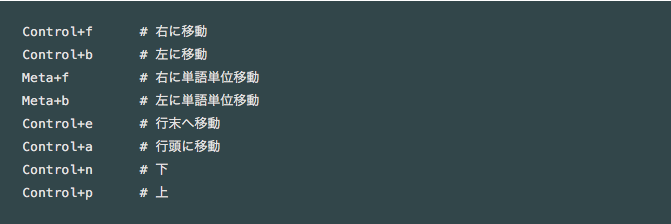
\includegraphics[width=150mm]{../../picture/keybind1.png}
\end{center}
\caption{カーソル移動系,\label{sample}}
\end{figure}

\begin{figure}[H]
\centering
\begin{center}
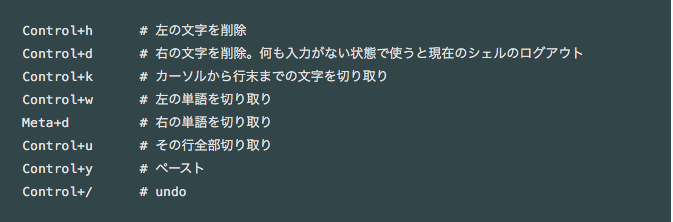
\includegraphics[width=150mm]{../../picture/keybind2.png}
\end{center}
\caption{文字操作系,\label{sample}}
\end{figure}

    \section{CUI(Character User
Interface)}\label{cuicharacter-user-interface}

CUIは,
\begin{quotation}
コンピュータにおいて,キーボード入力と文字表示のみを用いた,ソフトウェアの操作体系.キーボードのコマンド名を入力して操作する方法など. \cite{cui}
\end{quotation}

CUIとGUIにはそれぞれ大きな違いがある.GUIの利点は以下の通り,

\begin{itemize}
\tightlist
\item
  文字だけでなくアイコンなどの絵も表示できる.
\item
  対象物が明確な点や,マウスで比較的簡単に操作できる.
\item
  即座に操作結果が反映される.
\end{itemize}

CUIの利点は以下の通り,

\begin{itemize}
\tightlist
\item
  コマンドを憶えていれば複雑な処理が簡単に行える.
\item
  キーボードから手を離すことなく作業の高速化,効率化が行える.
\end{itemize}

今回GUIではなくCUI操作の習熟を目的にした理由は,

\begin{itemize}
\tightlist
\item
  コマンドを憶えることで作業効率が上がる.
\item
  editor操作の習熟も孕んでいるから.
\end{itemize}

カーソル移動においてもGUIではなくCUI操作により,ワンコマンドで動かした方が効率的である.プログラマにとってeditorを使わないことなどない.上記の理由から,GUIではなくCUI操作の習熟を目的としている.

    \section{使用したgemファイル}\label{ux4f7fux7528ux3057ux305fgemux30d5ux30a1ux30a4ux30eb}

    \subsection{diff-lcs}\label{diff-lcs}

    diff-lcsは,二つのファイルの差分を求めて出力してくれる.テキストの差分を取得するメソッドは,Diff::LCS.sdiffと Diff::LCS.diffの2つがある.複数行の文字列を比較した場合の2つのメソッドの違いは以下のとおり.

\begin{enumerate}
\def\labelenumi{\arabic{enumi}.}
\tightlist
\item
  Diff::LCS.sdiff

  \begin{enumerate}
  \def\labelenumii{\arabic{enumii}.}
  \tightlist
  \item
    比較結果を1文字ずつ表示する
  \end{enumerate}
\item
  Diff::LCS.diff

  \begin{enumerate}
  \def\labelenumii{\arabic{enumii}.}
  \tightlist
  \item
    比較した結果,違いがあった行について,違いがあった箇所のみ表示する.
  \end{enumerate}
\end{enumerate}

今回使用したのは後者(Diff:LCS.diff)である.コード自体が長いので全ての比較結果を表示してしまうとものすごく長くなってしまう.よって,違いがあった行のみの表示となっている.

    \subsection{Thor}\label{thor}

    Thorは,
\begin{quotation}
コマンドラインツールの作成を支援するライブラリです.gitやbundlerのようなサブコマンドツールを簡単に作成することができます. \cite{thor}
\end{quotation}
Thorの使用でサブコマンドを自然言語に近い形で設定できるので,非常にコマンドが覚えやすくなっている.

    \subsection{Minitest}\label{minitest}

    Minitestはテストを自動化するためのテスト用のフレームワークである.Rubyにはいくつかのテスティングフレームワークがありますが,Minitestというフレームワークを利用した理由は以下の通りです.

\begin{enumerate}
\def\labelenumi{\arabic{enumi}.}
\tightlist
\item
  Rubyをインストールすると一緒にインストールされるため,特別なセットアップが不要.
\item
  学習コストが比較的低い.
\item
  Railsのデフォルトのテスティングフレームワークなので,Railsを開発するときにも知識を活かしやすい.
\end{enumerate}

上記の理由から,sequential\_checkではminitestを採用しております.

    \subsection{FileUtils}\label{fileutils}

    再帰的な削除などの基本的なファイル操作を行うためのライブラリ今回使用したファイル操作は以下の通り.

\begin{enumerate}
\def\labelenumi{\arabic{enumi}.}
\tightlist
\item
 File.join: ファイルのパスとパスを結合する
\item
 File.exist: ファイルが存在するかどうかの判定.ファイルが存在して入れば"true"存在していなければ"false"を返り値としている.
\item
 FileUtils.mkdir\_p: ディレクトリdirとその親ディレクトリを全て作成する.
\item
 FileUtils.touch: パスに設定されているファイルを作成する.
\item
 FileUtils.cp: ファイルのコピーを行う.
\item
 File.expand\_path: パスを絶対パスに展開した文字列を返す.
\item
 FileUtils.compare\_file: 二つのファイルの比較を行う.一致して入れば"true"一致していなければ"false"を返り値としている.

\end{enumerate}

    \subsection{open3}\label{open3}

 open3は,
\begin{quotation}
プログラムを実行し,そのプロセスの標準入力,標準出力,標準出力にパイプをつなぎます. \cite{open3}
\end{quotation}

今回はopen3を利用してgemでinstallした場合にeditor\_learnerが格納されているパスを取得する.

    \subsection{Bundler}\label{bundler}

Bundlerは,
\begin{quotation}
gem同士の互換性を保ちながらパッケージの種類やバージョンを管理してくれる仕組みのことです.複数人,複数環境で開発を行う際に書く環境で扱うパッケージの種類やバージョンを合わせてくれる. \cite{bundler}
\end{quotation}


    \subsection{Rubocop}\label{rubocop}

RubocopはRubyのソースコード解析ツールである.Rubyスタイルガイドや他のスタイルガイドに準拠しているかどうかを自動チェックしてくれるソフトウェアです.自分が打ち込んだ問題文となるソースコードのチェックに使用した.
